\documentclass[12pt,a4paper]{article}
\usepackage[icelandic]{babel}
\usepackage[utf8]{inputenc}
\usepackage[T1]{fontenc}
\usepackage{hyperref}
\usepackage{verbatim}
\usepackage{fancyhdr}
\usepackage{tikz}
\usepackage{color}
\usepackage{datetime}

\usetikzlibrary{calc}
\usetikzlibrary{shapes}

\makeatletter
\setlength{\headheight}{15.2pt}
\pagestyle{fancy}

\newcommand{\myAlph}[1]{\char\numexpr`A-1+#1\relax}

% scrabble colours
\definecolor{x2word}{RGB}{255, 153, 255}
\definecolor{x3word}{RGB}{255,   0,   0}

\definecolor{x2letter}{RGB}{102, 204, 255}
\definecolor{x3letter}{RGB}{  0,  51, 255}

\newcommand{\coref}{\textbf{(Grunnkrafa)}}
\makeatother

\lhead{\textsc{Skrafl; Neo-deild}}
\rhead{\textsc{Háskólinn í Reykjavík}}

\title{Skrafl \\ \Large \textsc{Forritunarkeppni Framhaldsskólanna 2014 \\ Neo-deild}}
\author{Háskólinn í Reykjavík}
\newdate{date}{22}{03}{2014}
\date{\displaydate{date}}

\begin{document}

\maketitle

\begin{center}

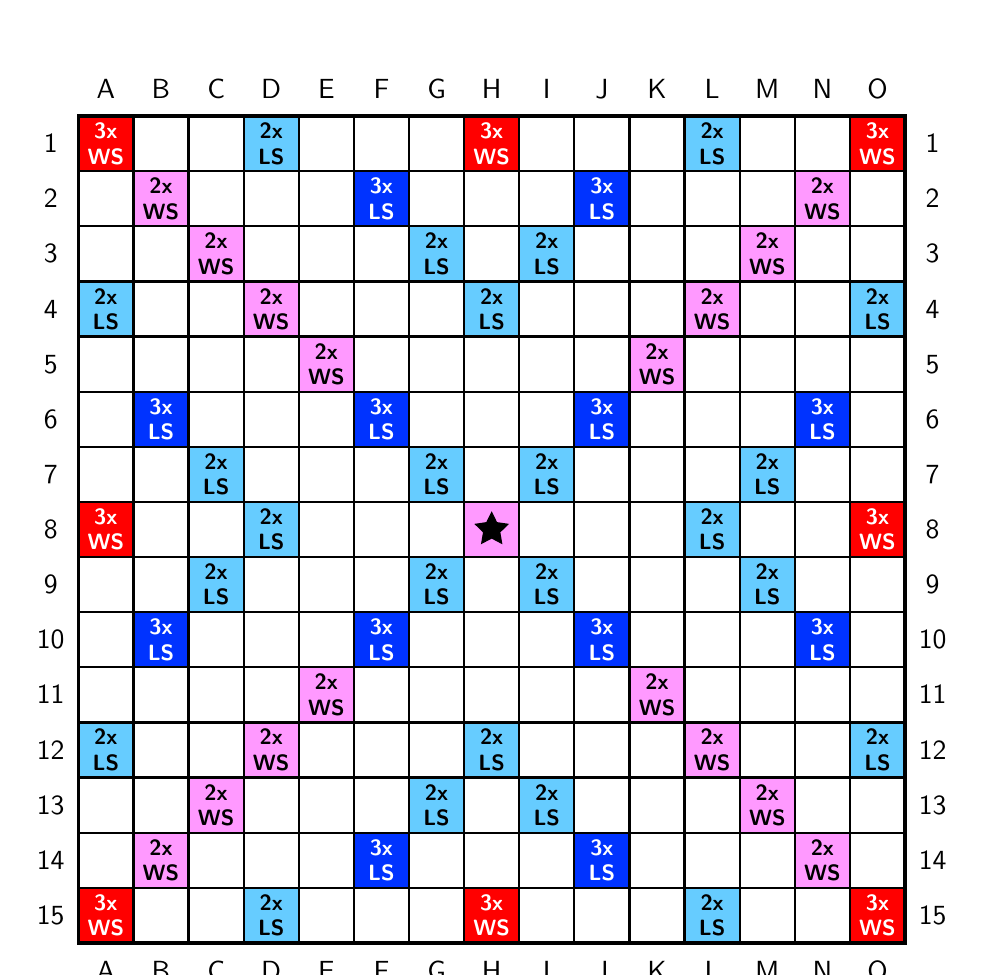
\begin{tikzpicture}[text depth=0pt, scale=0.7]
	% double word
	\foreach \x/\y in {
		 2/ 2,  3/ 3,  4/ 4,  5/ 5,
		14/ 2, 13/ 3, 12/ 4, 11/ 5,
		 2/14,  3/13, 4 /12, 5 /11,
		14/14, 13/13, 12/12, 11/11
	}{
		\fill[fill=x2word] (\x, 16-\y) rectangle (\x-1, 15-\y);
		\node at (\x-0.5, 15.73-\y) {\footnotesize \textsf{\textbf{2x}}};
		\node at (\x-0.5, 15.27-\y) {\footnotesize \textsf{\textbf{WS}}};
	}

	% tripple word
	\foreach \x/\y in {
		1/1, 15/15, 1/15, 15/1,
		8/1,  1/ 8, 8/15, 15/8
	}{
		\fill[fill=x3word] (\x, 16-\y) rectangle (\x-1, 15-\y);
		\node[color=white] at (\x-0.5, 15.73-\y) {\footnotesize \textsf{\textbf{3x}}};
		\node[color=white] at (\x-0.5, 15.27-\y) {\footnotesize \textsf{\textbf{WS}}};
	}

	% double letter
	\foreach \x/\y in {
		4/1, 12/1,
		7/3, 9/3,
		1/4, 8/4, 15/4,
		3/7, 7/7, 9/7, 13/7,
		4/8, 12/8,
		3/9, 7/9, 9/9, 13/9,
		1/12, 8/12, 15/12,
		7/13, 9/13,
		4/15, 12/15
	}{
		\fill[fill=x2letter] (\x, 16-\y) rectangle (\x-1, 15-\y);
		\node at (\x-0.5, 15.73-\y) {\footnotesize \textsf{\textbf{2x}}};
		\node at (\x-0.5, 15.27-\y) {\footnotesize \textsf{\textbf{LS}}};
	}

	% tripple letter
	\foreach \x/\y in {
		6/2, 10/2,
		2/6, 6/6, 10/6, 14/6,
		2/10, 6/10, 10/10, 14/10,
		6/14, 10/14
	}{
		\fill[fill=x3letter] (\x, 16-\y) rectangle (\x-1, 15-\y);
		\node[color=white] at (\x-0.5, 15.73-\y) {\footnotesize \textsf{\textbf{3x}}};
		\node[color=white] at (\x-0.5, 15.27-\y) {\footnotesize \textsf{\textbf{LS}}};
	}

	% center star
	\fill[fill=x2word] (8, 8) rectangle (7, 7);
	\node[star, star points=5, star point ratio=2, fill=black, scale=0.7] at (7.5, 7.5) {};

	\draw[very thick] (0, 0) rectangle (15, 15);
	\draw[thick, step=1.0] (0, 0) grid (15, 15);

	\foreach \i in {1,...,15}{
		\node at (-0.5, 16-\i-0.5) {\textsf{\i}};
		\node at (15.5, 16-\i-0.5) {\textsf{\i}};
		\node at (\i-0.5, -0.5) {\textsf{\myAlph{\i}}};
		\node at (\i-0.5, 15.5) {\textsf{\myAlph{\i}}};
	}
\end{tikzpicture}

\end{center}

\clearpage

\section*{Skrafl}

Í þessu verkefni á að útfæra leikinn Skrafl. Leikurinn Skrafl er spilaður á strjálu ferhyrndu leikborði. Í upphafi er leikmönnum úthlutað stafakubbum. Ætlunin er að leggja stafakubbana niður á leikborðið þannig að úr þeim myndast orð.

\subsection*{Leikborð}

\begin{itemize}

	\item Leikborðið skiptist í $15 \times 15$ reiti.

	\item Hver reitur rýmir einn stafakubb.

	\item Reiturinn innst í miðju (stjarnan) kallast upphafsreitur.

\end{itemize}

\subsection*{Stafakubbar}

\begin{itemize}

	\item Stafakubbarnir eru hundrað (100) talsins.

	\item Hver stafakubbur táknar staf úr enska stafrófinu. Aðeins er takmarkaður fjöldi kubba af hverjum staf.

	Tveir stafakubbana eru auðir. Þeir geta koma í stað fyrir alla aðra kubba.

	Skjalið \texttt{letter-distribution.txt} inniheldur tíðni stafanna.

	\item Stafakubbarnir gefa mismörg stig eftir hvaða staf þeir tákna. Til dæmis er stafurinn `E' mun algengari en `X', og gefur því færri stig. Auðir kubbar gefa engin stig.

	Skjalið \texttt{letter-values.txt} inniheldur upplýsingar um stigafjölda stafanna.

\end{itemize}

\subsection*{Leikreglur}

Hér fylgja leikreglur á Skrafli. Þær eru talsverðar, en þó er ekki nauðsynlegt að útfæra þær allar. Þeir þættir sem er mikilvægt að útfæra eru merktir sérstaklega með \coref{}.

\begin{itemize}

	\item \coref{} Áður en leikur hefst eru 100 stafakubbar geymdir í poka. Úr pokanum er hverjum leikmanni úthlutað sjö (7) kubbum hver. Leikmenn spila til skiptis.

	\item \coref{} Nú á fyrsti leikmaður sinn fyrsta leik. Lætur hann tvo eða fleiri af sínum stafakubbum af hendi og leggur þá á leikborðið.

	Stafirnir skulu vera samliggjandi og mynda orð þegar lesið er frá vinstri til hægri (vestri til austurs) eða toppi til botns (norðri til suðurs), eftir því hvernig orðið snýr. Einn af kubbunum skal liggja á upphafsreitnum.

	Skjalið \texttt{words.txt} inniheldur langan og fínan orðalista, en ekki er skylt að notast við þann lista.

	\item \coref{} Nú hefur leikmaður lokið leik. Dregur hann úr pokanum stafakubba þannig að hann hafi ávalt sjö (7) kubba á hendi. Skuli ekki vera nægilegur fjöldi kubba eftir í pokanum, situr leikmaðurinn eftir með færri kubba en ella.

	\item Nú á næsti leikmaður leik. Hefur hann nú möguleika á eitt af eftirfarandi aðgerðum:
	\begin{itemize}
		\item \coref{} Hann lætur einn eða fleiri stafakubba af hendi og leggur þá á leikborðið samliggjandi við önnur orð þegar mynduð, og myndar þar með ný orð.

		Allir kubbar lagðir niður þessa umferð verða að vera annaðhvort í sömu röð eða dálk. Liggja stafakubbarnir við aðra kubba í samliggjandi röðum eða dálkum, skulu þau öll einnig mynda lögleg orð.

		\item Hann skilar öllum eða sumum af sínum stafakubbum aftur í pokann, og dregur aðra af handahófi þannig að hann hafi sjö (7) stafakubba í hendi. Hann fær ekki að leggja út neina kubba þessa umferð.

		Leikmaður hefur frjálst val um hverjum af sínum kubbum skal skilað.

		\item Hann gerir ekkert þessa umferð.
	\end{itemize}

	\item Hefur leikmaður í höndum sínum auðan stafakubb, hefur hann kost á að nýta sér þann kubb eins og hver annar hefðbundinn kubbur. Þegar auði kubburinn er lagður á leikborðið, tilkynnir leikmaðurinn öðrum leikmönnum hvaða staf kubburinn skal tákna.

	Eftir að auður kubbur hefur verið lagður á leikborðið, má ekki breyta staf hans.

	\item \coref{} Leikur endar þegar annaðhvort allir hundrað stafakubbar hafa verið lagðir á leikborðið, eða þegar allar mögulegar hreyfingar hafa verið framkvæmdar.

\end{itemize}

\subsection*{Stigagjöf}

Stigagjöf í Skrafli er margþætt. Hér fylgja lýsingar á stigagjöfinni, en athugið að ekki er nauðsynlegt að útfæra alla þættina.

\begin{itemize}

	\item \coref{} Stigagjöf hvers leiks er summa stiga hvers stafakubbs í öllum orðum sem mynduð eru, eða breytast, í þeim leik.
	\begin{itemize}
		\item Auk þess bætast við stig sem fást fyrir að setja stafakubba á bónus\-reiti (athugið að þetta er ekki grunnkrafa).
	\end{itemize}

	\item Bónusreitur fyrir stafi: Ljósblár reitur tvöfaldar stigin sem fást fyrir stafakubbinn sem settur er á þann reit; dökkblár reitur þrefaldar stigin.

	\item Bónusreitur fyrir orð: Stigin sem fást fyrir heilt orð eru tvöfölduð þegar einn af stafakubbunum er settur á bleikan reit en rauður reitur þrefaldar stigin. Takið með bónusa fyrir stafi, ef einhverjir, áður en þið reiknið bónusa fyrir orð. Ef orð hylur tvo bónusreiti, þá eru stigin tvöfölduð og tvöfölduð aftur (eða þrefölduð og þrefölduð aftur ef bónus\-reitirnir eru rauðir).

	Athugið að miðjureiturinn er bleikur, og eru því stigin fyrir fyrsta orðið tvöfölduð.

	\item Aðeins fást aukastig fyrir bónusreiti í þeim leik þegar stafakubbar eru lagðir á þá. Í seinni umferðum fást engin aukastig fyrir stafakubba á bónusreitum.

	\item Þegar auðu stafakubbarnir eru settir á bleika eða rauða reiti eru stig orðsins tvöfölduð, eða þrefölduð, jafnvel þó að auði stafakubburinn gefi engin stig.

	\item \coref{} Þegar tvö eða fleiri orð eru mynduð í einum leik, þá eru stig allra orðanna lögð saman. Stafir sem orð eiga sameiginlega eru taldir fyrir sérhvert orð (með öllum bónusstigum sem við á).

	\item Að leika 7 stafakubbum í einum leik kallast Bingó. Ef leikmaður leikur bingó, bætast 50 stig við eftir að stig leiksins hafa verið talin.

	\item Þegar leik lýkur er summa stafakubba hvers leikmanns dregin frá heildarstigum hans. Ef leikmaður hefur notað alla sína stafakubba í lok leiks, þá er summa stafakubba allra annarra leikmanna lögð við stig hans.

	\item \coref{} Sá leikmaður sem hefur flest stig vinnur leikinn. Ef upp kemur jafntefli, þá vinnur sá leikmaður sem var með flest stig áður en stig voru lögð við, eða dregin frá, fyrir óleikna stafakubba.

\end{itemize}

\subsection*{Aukavirkni}

Hér koma hugmyndir að aukinni virkni leiksins. Ykkur er frjálst (og þið eruð hvött til þess) að útfæra ykkar eigin hugmyndir.

\begin{itemize}

	\item Gera grafískt viðmót fyrir leikinn. Þetta getur t.d.~verið gluggaviðmót eða vefviðmót.

	\item Búa til miðlara (e.~server) sem að gerir tveimur, eða fleiri, leikmönnum kleift að spila leikinn samtímis.  Þá væri hægt að hafa anddyri þar sem leikmenn hittast og spjalla saman, og geta svo óskað eftir að spila við aðra leikmenn.

	\item Mismunandi stærðir af leikborðum.

	\item Íslensk útfærsla; með íslenskum stöfum, orðalista, og stigagjöf. Einnig væri hægt að bæta við fleiri tungumálum og leyfa notanda að velja.

	\item Tæknibrellur, eins og hreyfimyndir og hljóð (tónlist).

	\item Halda utan um leikmenn í gagnagrunni. Geyma upplýsingar um spilaða leiki, stig hvers leikmanns, og jafnvel setja upp stigatöflu.

	\item Gefa leikmönnum ábendingar um góða leiki á kostnað stiga.

\end{itemize}

\end{document}
